\noindent Based on the deviations of simulation viscosity from empirical predictions, the potential source of the deviation could be due to the branch length. Hence, we now focus our attention on the importance of branch length for $\mu_{app}$ estimations. However, instead of directly characterising $\mu_{rel}$ against the measure of the absolute branch length ($L$), another parameter called distance ratio (ratio of branch length to branch diameter) was considered with a classification of "in vivo favoured" and "in vitro favoured" branches. The evaluated deviations between simulation data against \textit{in vivo} and \textit{in vitro} empirical predictions are represented as vivo-ERR and vitro-ERR respectively. 

\begin{figure}[H]
\centering
\begin{subfigure}{0.45 \textwidth}
    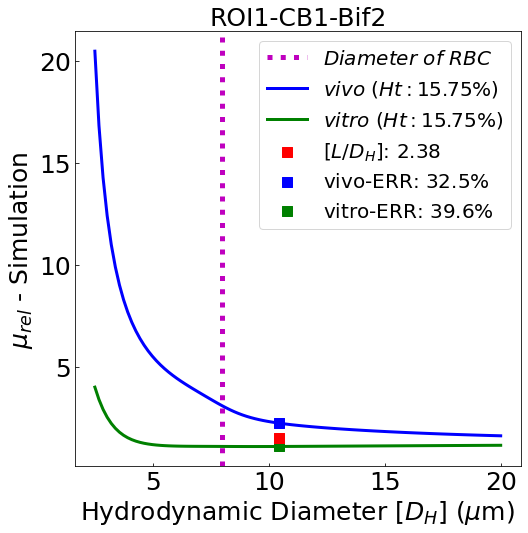
\includegraphics[width=0.92\textwidth]{images/DeviationsViscosity1.png}
    \caption{\textit{} \label{DeviationsViscosity1}}
\end{subfigure}
\hfill
\begin{subfigure}{0.45 \textwidth}
    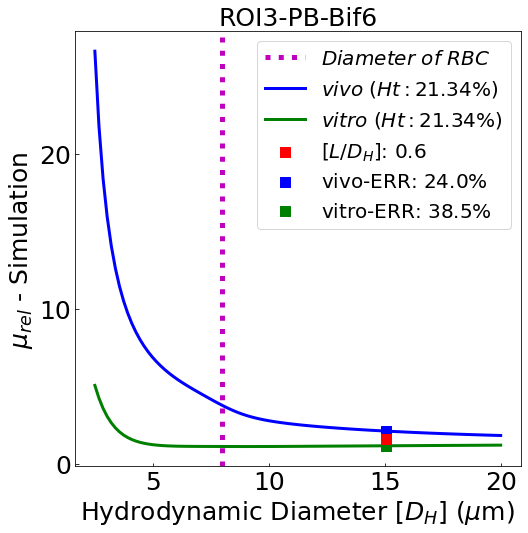
\includegraphics[width=0.92\textwidth]{images/DeviationsViscosity2.png}
    \caption{\textit{} \label{DeviationsViscosity2}}
\end{subfigure}
\hfill
\begin{subfigure}{0.45 \textwidth}
    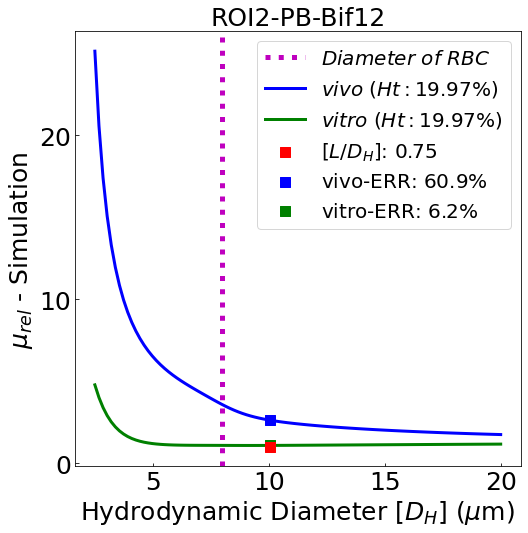
\includegraphics[width=0.92\textwidth]{images/DeviationsViscosity3.png}
    \caption{\textit{} \label{DeviationsViscosity3}}
\end{subfigure}
\hfill
\begin{subfigure}{0.45 \textwidth}
    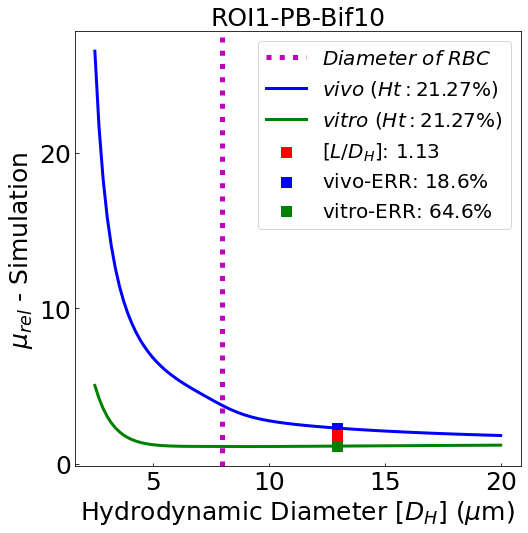
\includegraphics[width=0.92\textwidth]{images/DeviationsViscosity4.png}
    \caption{\textit{} \label{DeviationsViscosity4}}
\end{subfigure}
\caption{\textit{Comparison of simulation data (red) against empirical predictions of both Pries Viscosity Models (blue and green) within studied networks. The solid lines represent the empirical models and the purple dotted line indicates the average RBC diameter. (a$-$b) Exemplar individual branches with simulation data in-between empirical predictions. (c$-$d) Examples of "in vitro favoured" and "in vivo favoured" branches respectively.} \label{DeviationsVisocity}}
\end{figure}

\noindent Kindly note that the context of "in vivo favoured" and "in vitro favoured" is a relative notion between the vivo-ERR and vitro-ERR in each branch. This means if vivo-ERR $>$ vitro-ERR in a given branch, that branch is "in vitro favoured" (whereas the branch is "in vivo favoured" if vivo-ERR $<$ vitro-ERR). Based on this assessment, we hypothesized that the smaller distance ratio ($L$/D$_{H}$) branches should match relatively better with \textit{in vivo} formulation instead of \textit{in vitro} formulation. \\

\noindent In addition to this, it was previously mentioned in Section \ref{Fahraeus_Lindqvist_Effect} that the $\mu_{app}$ values evaluated from simulation data appear to be in-between the empirical predictions from both Pries Viscosity Models (\textit{in vitro} and \textit{in vivo}). To justify this claim, simulation data with non-zero haematocrit in each individual branch were compared to the empirical predictions from both \textit{in vitro} and \textit{in vivo} formulations. The results for the individual branches in ROI1, ROI2 and ROI3 are listed in Appendix \ref{EvaluationOfSimulationDataVSPVM} (see Figures \ref{DeviationsViscosity-ROI1}$-$\ref{DeviationsViscosity-ROI3}). The results indicated 29 branches out of 57 were classified as "in vitro favoured" while the remaining 28 branches were "in vivo favoured". An illustration of 4 individual branches is presented (see Figure \ref{DeviationsVisocity}) for which the first 2 examples indicate the actual apparent viscosity was somewhere between both Pries Viscosity Models while the last 2 examples show the classification of "\textit{in vitro} favoured" and "\textit{in vivo} favoured" branches. 


\begin{figure}[H]
\centering
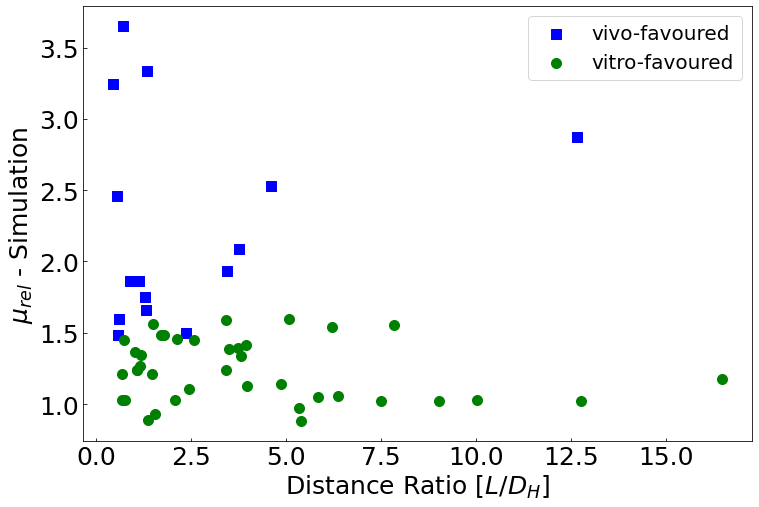
\includegraphics[width=0.75\textwidth]{images/RelativeApparentViscosityVSDistanceRatio.png}
\caption{\textit{Correlation between relative apparent blood viscosity against distance ratio} \label{RelativeApparentViscosityVSDistanceRatio}}
\end{figure}

\noindent From Figure \ref{RelativeApparentViscosityVSDistanceRatio}, it was observed that majority of the "\textit{in vivo} favoured" branches have a variation of $\mu_{rel}$ (ranging from 1.3 up to 3.6) for a given distance ratio. Whereas for "\textit{in vitro} favoured" branches, it was noticed to have a relatively constant $\mu_{rel}$ (limited up to around 1.5) across the entire range of distance ratios. It was also apparent that the range of distance ratio for "\textit{in vivo} favoured" branches excluding one single outlier was found within 0 to 5 while it was across the whole range for "\textit{in vitro} favoured" branches. These findings concur with the initial hypothesis whereby the smaller $L$/D$_{H}$ branches are usually better matched with the \textit{in vivo} formulation of Pries Viscosity Model where "\textit{in vivo} favoured" branches lie within a distinct range unlike "\textit{in vitro} favoured" branches. Therefore, this highlights the importance of considering the branch length for $\mu_{app}$ estimation because the majority of the branches from simulation data are relatively shorter compared to the extended glass tubes for the \textit{in vitro} model and the long vessels for the \textit{in vivo} model. \\


\noindent Another apparent observation found in Figure \ref{RelativeApparentViscosityVSDistanceRatio} was the inverse relationship between $\mu_{rel}$ and distance ratio which also implies that short branches tend to have a higher relative apparent blood viscosity. A similar way of describing this is that the apparent blood viscosity ($\mu_{app}$) in any branch will increase when the branch length ($L$) decreases. This is an interesting result observed as it is not something that can be observed from Hagen-Poiseuile's equation (correlation between $\mu_{app}$ and $L$). Also, under Poiseuille's law, a fully developed flow is assumed as the effects of the conditions at the entrance of each branch were neglected. Therefore, a plausible reason behind this observation could be due to the entrance effect where it requires more energy for the RBCs to move into the branch, but once the RBCs are inside the branch, it seems easier for the RBCs to continue flowing. This shows that a closer look at the correlation between $L$ and D$_{H}$ will be required to disentangle their contributions on the $\mu_{app}$ which influences the asymmetric RBC distribution across micro-vascular networks. \\

\noindent In addition to this, the dependence of $\lvert Q^{*}_{rbc} - Q^{*}_{blood} \rvert$ on the distance ratio was also considered (see Figure \ref{DisproportionalityIndexDistanceRatio}). Following the practice of Balogh and Bagchi\cite{Balogh2018}, the quantity of $\lvert Q^{*}_{rbc} - Q^{*}_{blood} \rvert$ was considered as a measure of disproportionality in RBC partitioning. With reference to this, it was observed that the $\lvert Q^{*}_{rbc} - Q^{*}_{blood} \rvert$ value increases with decreasing distance ratio. Furthermore, we have noticed that across the studied networks, shorter branches tend to have a relatively larger diameter (and vice versa) within a given bifurcation. This suggests that on average the RBC partitioning tend to become less disproportionate as the branch length increases. However, this might not be true given that $L$/D$_{H}$ will always have a tendency to become smaller with increasing D$_{H}$, unless the length of a branch grows more strongly than D$_{H}$. Therefore, understanding the correlation between $L$ and D$_{H}$ will help justify the influence of $L$/D$_{H}$ onto the degree of disproportionality in RBC partitioning.\\



\begin{figure}[H]
\centering
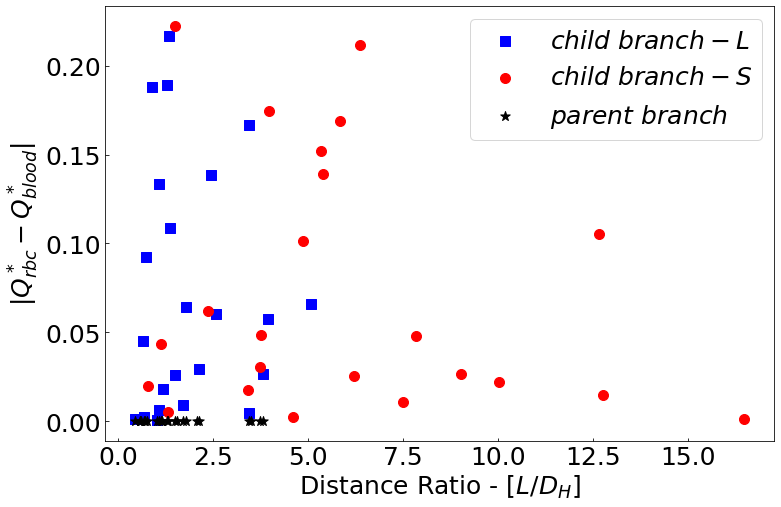
\includegraphics[width=0.75\textwidth]{images/DisproportionalityIndexDistanceRatio.png}
\caption{\textit{Influence of the distance ratio on the degree of disproportionality in RBC partitioning. The "L"/"S" indicate the relatively larger (blue squares) and smaller (red circles) child branches in each diverging bifurcation respectively.} \label{DisproportionalityIndexDistanceRatio}}
\end{figure}